\subsection{THE COMPLETION OF A UNIFORM SPACE}

THEOREM 3. Let X be a uniform space. Then there exists a complete Hausdorff uniform space \(\hat{\mathbf{X}}\) and a uniformly continuous mapping \(i: \mathbf{X} \to \hat{\mathbf{X}}\) having the following property:

\begin{enumerate}
\def\labelenumi{(\Alph{enumi})}
\setcounter{enumi}{15}
\tightlist
\item
  Given any uniformly continuous mapping \(f\) of \(\mathbf{X}\) into a complete Hausdorff uniform space \(\mathbf{Y}\) , there is a unique uniformly continuous mapping \(g: \hat{\mathbf{X}} \to \mathbf{Y}\) such that \(f = g \circ i\) .
\end{enumerate}

If \((i_1, X_1)\) is another pair consisting of a complete Hausdorff uniform space \(X_1\) and a uniformly continuous mapping \(i_1: X \to X_1\) having the property (P), then there is a unique isomorphism \(\varphi: \hat{X} \to X_1\) such that \(i_1 = \varphi \circ i\) .

The first statement of the theorem signifies that the pair \((i, \hat{\mathbf{X}})\) is the solution of the universal mapping problem (Set Theory, Chapter IV, § 3, no. 1) in which the \(\Sigma\) -sets are complete Hausdorff uniform spaces, the \(\sigma\) -morphisms are uniformly continuous mappings and the \(\alpha\) -mappings are uniformly continuous mappings of X into a complete Hausdorff uniform space. The uniqueness of the pair \((i, \hat{\mathbf{X}})\) up to a unique isomorphism therefore follows from the general properties of solutions of universal mapping problems (loc. cit.). It remains to prove the existence of the pair \((i, \hat{\mathbf{X}})\) .

\begin{enumerate}
\def\labelenumi{\arabic{enumi})}
\tightlist
\item
  Definition of \(\hat{\mathbf{X}}\) . Let \(\hat{\mathbf{X}}\) be the set of minimal Cauchy filters (no. 2) on \(\mathbf{X}\) . We shall define a uniform structure on \(\hat{\mathbf{X}}\) . For this purpose, if \(\mathbf{V}\) is any symmetric entourage of \(\mathbf{X}\) , let \(\tilde{\mathbf{V}}\) denote the set of all pairs \((\mathfrak{X}, \mathfrak{Y})\) of minimal Cauchy filters which have in common a V-small set. We shall show that the sets \(\tilde{\mathbf{V}}\) form a fundamental system of entourages of a uniform structure on \(\hat{\mathbf{X}}\) :
\end{enumerate}

\begin{enumerate}
\def\labelenumi{(\roman{enumi})}
\item
  Since each \(\mathcal{X} \in \hat{\mathbf{X}}\) is a Cauchy filter, we have by definition \((\mathcal{X}, \mathcal{X}) \in \tilde{\mathbf{V}}\) for every symmetric entourage \(\mathbf{V}\) of \(\mathbf{X}\) ; hence axiom \((\mathbf{U}_{\mathbf{I}}^{\prime})\) is satisfied.
\item
  If V and \(V'\) are two symmetric entourages of X, then \(W = V \cap V'\) is a symmetric entourage, and every set which is W-small is also V-small and \(V'\) -small; hence \(\tilde{W} \subset \tilde{V} \cap \tilde{V}'\) , which prove \((B_{I})\) .
\item
  The sets \(\tilde{\mathbf{V}}\) are symmetric by definition, hence \((\mathbf{U}_{\mathbf{II}}^{\prime})\) is satisfied. (iv) Given a symmetric entourage \(\mathbf{V}\) of \(\mathbf{X}\) , let \(\mathbf{W}\) be a symmetric entourage such that \(\tilde{\mathbf{V}} \subset \mathbf{V}\) . Consider three minimal Cauchy filters \(\mathcal{X}, \mathcal{Y}, \mathfrak{Z}\) such that \((\mathcal{X}, \mathcal{Y}) \in \tilde{\mathbf{W}}\) and \((\mathcal{Y}, \mathfrak{Z}) \in \tilde{\mathbf{W}}\) ; then there are two W-small sets \(\mathbf{M}, \mathbf{N}\) such that \(\mathbf{M} \in \mathcal{X} \cap \mathcal{Y}\) and \(\mathbf{N} \in \mathcal{Y} \cap \mathfrak{Z}\) . Since \(\mathbf{M}\) and \(\mathbf{N}\) belong to \(\mathcal{Y}\) , \(\mathbf{M} \cap \mathbf{N}\) is not empty and therefore (no. 1, Proposition 1) \(\mathbf{M} \cup \mathbf{N}\) is \(\tilde{\mathbf{W}}\) -small and hence V-small; since \(\mathbf{M} \cup \mathbf{N}\) belongs to \(\mathcal{X}\) and to \(\mathfrak{Z}\) we have \(\tilde{\mathbf{W}} \subset \tilde{\mathbf{V}}\) ; hence \((\mathbf{U}_{\mathbf{III}}^{\prime})\) is satisfied.
\end{enumerate}

We show next that the uniform space \(\hat{\mathbf{X}}\) is Hausdorff. Let \(\mathcal{X},\mathcal{Y}\) be two minimal Cauchy filters on \(\mathbf{X}\) such that \((\mathcal{X},\mathcal{Y})\in \hat{\mathbf{X}}\) for all symmetric entourages \(\mathbf{V}\) of \(\mathbf{X}\) . It follows immediately that the sets \(\mathbf{M}\cup \mathbf{N}\) , where \(\mathbf{M}\in \mathcal{X}\) and \(\mathbf{N}\in \mathcal{Y}\) , form a base of a filter \(\mathfrak{Z}\) coarser than \(\mathcal{X}\) and \(\mathcal{Y}\) . Now \(\mathfrak{Z}\) is a Cauchy filter, since for every symmetric entourage \(\mathbf{V}\) of \(\mathbf{X}\) there is by hypothesis a V-small set \(\mathbf{P}\) belonging to both \(\mathcal{X}\) and \(\mathcal{Y}\) and therefore belonging to \(\mathfrak{Z}\) . By the definition of minimal Cauchy filters, we have \(\mathcal{X} = \mathfrak{Z} = \mathcal{Y}\) , and this shows that \(\hat{\mathbf{X}}\) is Hausdorff.

\begin{enumerate}
\def\labelenumi{\arabic{enumi})}
\setcounter{enumi}{1}
\item
  Definition of \(i\) ; the uniform structure of \(\mathbf{X}\) is the inverse image under \(i\) of that of \(\hat{\mathbf{X}}\) . We know that for each \(x \in \mathbf{X}\) the neighbourhood filter \(\mathfrak{B}(x)\) of \(x\) in \(\mathbf{X}\) is a minimal Cauchy filter (no. 2, Proposition 5, Corollary 1). So we define \(i(x) = \mathfrak{B}(x)\) . Let \(f = i \times i\) ; we shall show that for each symmetric entourage \(\mathbf{V}\) of \(\mathbf{X}\) we have \(\overline{j}(\tilde{\mathbf{V}}) \subset \mathbf{V} \cup \overline{j}[(\mathbf{V})^{\sim}]\) , and this will prove our assertion (§ 2, no. 4). Now, if \([i(x), i(y)] \in \tilde{\mathbf{V}}\) , there is a V-small set \(\mathbf{M}\) which is a neighbourhood of each of \(x\) and \(y\) , hence \((x, y) \in \mathbf{V}\) . Conversely, if \((x, y) \in \mathbf{V}\) , it is immediately seen that the set \(\mathbf{V}(x) \cup \mathbf{V}(y)\) is \(\overline{\mathbf{V}}\) -small and is a neighbourhood of each of \(x\) and \(y\) .
\item
  \(\hat{\mathbf{X}}\) is complete and \(i(\mathbf{X})\) is dense in \(\hat{\mathbf{X}}\) . The trace on \(i(\mathbf{X})\) of a neighbourhood \(\tilde{\mathbf{V}}(\mathfrak{X})\) of a point \(\mathfrak{X} \in \hat{\mathbf{X}}\) is the set of all \(i(x)\) such that
\end{enumerate}

\[
(\mathcal {X}, i (x)) \in \tilde {\mathbf {V}}.
\]

This relation means that there is a V-small neighbourhood of \(x\) in X which belongs to \(\mathcal{X}\) , i.e.~that \(x\) is an interior point of a V-small set of \(\mathcal{X}\) . Let M be the union of the interiors of all V-small sets of \(\mathcal{X}\) ; then M belongs to \(\mathcal{X}\) (no. 2, Proposition 5, Corollary 4) and from what has been said it follows that \(\tilde{\mathrm{V}}(\mathcal{X}) \cap i(\mathrm{X}) = i(\mathrm{M})\) . We conclude that:

\begin{enumerate}
\def\labelenumi{(\roman{enumi})}
\item
  \(\tilde{\mathbf{V}}(\mathcal{X}) \cap i(\mathbf{X})\) is not empty, hence \(i(\mathbf{X})\) is dense in \(\hat{\mathbf{X}}\) .
\item
  The trace of \(\tilde{\mathbf{V}}(\mathcal{X})\) on \(i(\mathbf{X})\) belongs to the filter base \(i(\mathcal{X})\) on X; hence this filter base converges in \(\hat{X}\) to the point \(\mathfrak{X}\).
\end{enumerate}

Now let \(\mathfrak{F}\) be a Cauchy filter on \(i(\mathbf{X})\) ; then from 2) above and Proposition 4 of no. 1, \(\overline{i}^{1}(\mathfrak{F})\) is a base of a Cauchy filter \(\mathfrak{G}\) on \(\mathbf{X}\) . Let \(\mathfrak{X}\) be a minimal Cauchy filter coarser than \(\mathfrak{G}\) (no. 2, Proposition 5); then \(i(\mathfrak{X})\) is a Cauchy filter base on \(i(\mathbf{X})\) (no. 1, Proposition 3), and \(\mathfrak{F}=i[\overline{i}^{1}(\mathfrak{F})]\) is finer than the filter whose base is \(i(\mathfrak{X})\) . Since the latter converges in \(\hat{\mathbf{X}}\) , so does \(\mathfrak{F}\) , and Proposition 9 of no. 4 therefore shows that \(\hat{\mathbf{X}}\) is complete.

\begin{enumerate}
\def\labelenumi{\arabic{enumi})}
\setcounter{enumi}{3}
\tightlist
\item
  Verification of the property (P). Let \(f\) be a uniformly continuous mapping of \(\mathbf{X}\) into a complete Hausdorff uniform space \(\mathbf{Y}\) . Let us first show that there is a unique uniformly continuous mapping \(g_{0}: i(\mathbf{X}) \to \mathbf{Y}\) such that \(f = g_{0} \circ i\) . Since \(f\) is continuous, we have
\end{enumerate}

\[
f (x) = \lim f (\mathfrak {B} (x)),
\]

hence if we put \(g_0(i(x)) = \lim f(\mathfrak{V}(x))\) , we have \(f = g_0 \circ i\) ; so it remains to show that \(g_0\) is uniformly continuous in \(i(\mathbf{X})\) . Let \(\mathbf{U}\) be an entourage of \(\mathbf{Y}\) and let \(\mathbf{V}\) be a symmetric entourage of \(\mathbf{X}\) such that the relation \((x, x') \in \mathbf{V}\) implies \((f(x), f(x')) \in \mathbf{U}\) ; we have seen in 2) that the relation \((i(x), i(x')) \in \tilde{\mathbf{V}}\) implies \((x, x') \in \mathbf{V}\) , hence also is implied

\[
(g _ {0} (i (x)), g _ {0} (i (x ^ {\prime}))) \in \mathbf {U},
\]

which proves our assertion.

Let \(g\) be the extension of \(g_0\) by continuity to \(\hat{\mathbf{X}}\) (no. 6, Theorem 2); then \(f = g \circ i\) , and it is clear that \(g\) is the unique continuous mapping of \(\hat{\mathbf{X}}\) into \(Y\) satisfying this relation, since \(i(\mathbf{X})\) is dense in \(\hat{\mathbf{X}}\) (Chapter I, § 8, no. 1, Proposition 2, Corollary 1).

Q.E.D.

DEFINITION 4. The complete Hausdorff uniform space \(\hat{\mathbf{X}}\) defined in the proof of Theorem 3 is called the Hausdorff completion of \(\mathbf{X}\) , and the mapping \(i: \mathbf{X} \to \hat{\mathbf{X}}\) is called the canonical mapping of \(\mathbf{X}\) into its Hausdorff completion.

We note also the following facts:

PROPOSITION 12. (i) The subspace \(i(\mathbf{X})\) is dense in \(\hat{\mathbf{X}}\) .

\begin{enumerate}
\def\labelenumi{(\roman{enumi})}
\setcounter{enumi}{1}
\item
  The graph of the equivalence relation \(i(x) = i(x')\) is the intersection of the entourages of \(\mathbf{X}\) .
\item
  The uniform structure of X is the inverse image under i of that of \(\hat{X}\) {[}or of that of the subspace \(i(\mathbf{X})\) {]}.
\item
  The entourages of \(i(\mathbf{X})\) are the images under \(i \times i\) of the entourages of X, and the closures in \(\hat{X} \times \hat{X}\) of the entourages of \(i(\mathbf{X})\) form a fundamental system of entourages of \(\hat{X}\) .
\item
  and (iii) have been proved in the course of the proof of Theorem 3; (iv) is a consequence of (i) and (iii) by virtue of general results proved earlier (§ 2, no. 4, Remark and Proposition 6). The relation
\end{enumerate}

\[
i (x) = i \left(x ^ {\prime}\right)
\]

means by definition that \(x\) and \(x'\) have the same neighbourhood filter. But this implies, by definition, that \((x, x') \in V\) for every entourage \(V\) of \(X\) , and the converse is obvious.

COROLLARY. If X is a Hausdorff uniform space, then the canonical mapping \(i: X \to \hat{X}\) is an isomorphism of X onto a dense subspace of \(\hat{X}\) .

When X is Hausdorff, \(\hat{X}\) is said to be the completion of X, and we generally identify X with a dense subset of \(\hat{X}\) by means of i.

Remark. If this identification is made, the minimal Cauchy filters on X are just the traces on X of the neighbourhood filters of points of \(\hat{X}\) ; this follows from the proof of Theorem 3.

The Corollary to Proposition 12 characterizes the completion of a Hausdorff uniform space:

PROPOSITION 13. If Y is a complete Hausdorff uniform space and X a dense subspace of Y, then the canonical injection \(\mathbf{X} \to \mathbf{Y}\) extends to an isomorphism of \(\hat{\mathbf{X}}\) onto Y.

For every uniformly continuous mapping of X into a complete Hausdorff uniform space Z extends uniquely to a uniformly continuous mapping of Y into Z by Theorem 2 of no. 6.

PROPOSITION 14. Let X be a complete Hausdorff uniform space, U its uniformity, and let Z be a dense subspace of X. If U' is a uniformity on X which is coarser than U and which induces the same uniformity as U on Z, then U = U'.

Let \(X'\) denote the set \(X\) with the uniformity \(\mathcal{U}'\) . The composition of the canonical mapping \(X' \to \hat{X}'\) and the identity mapping \(X \to X'\) is a uniformly continuous mapping \(\varphi: X \to \hat{X}'\) . Since \(Z\) is Hausdorff for the uniform structure induced by \(\mathcal{U}'\) , the restriction of \(\varphi\) to \(Z\) is by hypothesis an isomorphism of \(Z\) onto the dense subspace \(\varphi(Z)\) of \(\hat{X}'\) ; it follows (no. 6, Corollary to Theorem 2) that \(\varphi\) itself is an isomorphism of \(X\) onto \(\hat{X}'\) , hence \(X' = \hat{X}'\) and \(\mathcal{U}' = \mathcal{U}\) .

PROPOSITION 15. Let X and X' be two uniform spaces. For each uniformly continuous mapping \(f: \mathbf{X} \to \mathbf{X}'\) there is a unique uniformly continuous mapping \(\hat{f}: \hat{\mathbf{X}} \to \hat{\mathbf{X}}'\) such that the diagram

\[
\begin{array}{c}\mathbf {X} \stackrel {{i ^ {\prime}}} {{\to}} \mathbf {X} ^ {\prime}\\i \downarrow \quad \quad \quad \quad \quad \quad \quad \quad \quad \quad \quad \quad \quad \quad \quad \quad \quad \quad \quad \quad \hat {\mathbf {X}} \stackrel {{\rightarrow}} {{\longrightarrow}} \hat {\mathbf {X}} ^ {\prime}\\f\end{array}
\]

is commutative (*), where \(i: \mathbf{X} \to \hat{\mathbf{X}}\) and \(i': \mathbf{X}' \to \hat{\mathbf{X}}'\) are the canonical mappings.

Apply Theorem 3 to the function \(i' \circ f: \mathbf{X} \to \hat{\mathbf{X}}'\) .

COROLLARY. If \(f: \mathbf{X} \to \mathbf{X}'\) and \(g: \mathbf{X}' \to \mathbf{X}''\) are two uniformly continuous mappings and \(h = g \circ f\) , then \(\hat{h} = \hat{g} \circ \hat{f}\) .

This is an immediate consequence of the uniqueness in Proposition 15.

\subsection{THE HAUSDORFF UNIFORM SPACE ASSOCIATED WITH A UNIFORM SPACE}

PROPOSITION 16. Let X be a uniform space and i the canonical mapping of X into its Hausdorff completion \(\hat{\mathbf{X}}\) . For each uniformly continuous mapping \(f\) of X into a Hausdorff uniform space Y, there is a unique uniformly continuous mapping \(h: i(\mathbf{X}) \to \mathbf{Y}\) such that \(f = h \circ i\) .

We may identify Y with a subspace of its completion \(\hat{Y}\) (no. 7, Corollary to Proposition 12), and f can then be considered as a uniformly continuous mapping of X into \(\hat{Y}\) . By virtue of Theorem 3, f is then of the form \(f = g \circ i\) , where g is a uniformly continuous mapping of \(\hat{X}\) into \(\hat{Y}\) . If h is the restriction of g to \(i(X)\) , then clearly \(f = h \circ i\) , and h maps \(i(X)\) into Y. The uniqueness of h is trivial.

The pair \((i, i(X))\) is therefore the solution of a universal mapping problem (Set Theory, Chapter IV, § 3, no. 1), where this time we take the \(\Sigma\) -sets to be Hausdorff uniform spaces, and the \(\sigma\) -morphisms (resp. \(\alpha\) -mappings) to be uniformly continuous mappings (resp. uniformly continuous mappings of X into a Hausdorff uniform space).

DEFINITION 5. The Hausdorff uniform space \(i(\mathbf{X})\) defined in the proof of Theorem 3 is called the Hausdorff uniform space associated with \(\mathbf{X}\) .

The Hausdorff completion of X is thus the completion of the Hausdorff uniform space associated with X.

COROLLARY. Let X, Y be two uniform spaces and \(X'\) , \(Y'\) the associated Hausdorff spaces. For each uniformly continuous mapping \(f: X \to Y\) there is a unique uniformly continuous mapping \(f': X' \to Y'\) for which the diagram

\pandocbounded{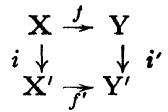
\includegraphics[keepaspectratio]{images/part002_3c8eaa6f.jpg}}

is commutative, where \(i\) and \(i'\) are the canonical mappings.

Apply Proposition 16 to \(i' \circ f: \mathbf{X} \to \mathbf{Y}'\) .

The Hausdorff space associated with a uniform space may also be characterized by the following property:

PROPOSITION 17. Let X be a uniform space, \(i(X)\) its associated Hausdorff space, and let \(f\) be a mapping of X onto a Hausdorff uniform space \(X'\) , such that the uniformity of X is the inverse image under \(f\) of the uniformity of \(X'\) . Then the mapping \(g:i(X)\to X'\) such that \(f=g\circ i\) is an isomorphism.

By Proposition 16, g is uniformly continuous; also g is obviously surjective, and is also injective because the relation \(f(x) = f(y)\) implies by definition that \((x,y)\) belongs to all the entourages of X, and therefore that \(i(x)=i(y)\) (no. 7, Proposition 12). Finally, the entourages of \(X'\) are the images under \(f\times f\) of the entourages of X (§ 2, no. 4, Remark), hence they are also the images under \(g\times g\) of the entourages of \(i(\mathbf{X})\) (no. 7, Proposition 12); hence the result.

Remark. Let R be the equivalence relation \(i(x) = i(x')\) on X. We have seen (no. 7, Proposition 12) that the graph C of R is the intersection of all the entourages of X. It is clear that every open set (and therefore also every closed set) in X is saturated with respect to R; taking account of the definition of the inverse image of a topology, we conclude that the canonical bijection of the quotient space X/R onto \(i(X)\) induced by \(i\) is a homeomorphism. The Hausdorff space associated with X can therefore be identified, qua topological space, with X/R. The canonical mapping \(i: X \to i(X)\) is open and closed, and even proper (Chapter I, § 10, no. 2, Example).

Let \(X'\) be another uniform space, \(C'\) the intersection of all the entourages of \(X'\) , and \(R'\) the equivalence relation whose graph is \(C'\) . Let \(f: X \to X'\) be a continuous mapping. Since the inverse image under \(f\) of any neighbourhood of \(f(x)\) is a neighbourhood of \(x\) , it follows that the inverse image under \(f\) of \(C'(f(x))\) contains \(C(x)\) , and therefore \(f\) is compatible with \(R\) and \(R'\) , and induces a continuous mapping \(X/R \to X'/R'\) (Chapter I, § 3, no. 4, Corollary to Proposition 6). This generalizes the corollary to Proposition 16.

\subsection{COMPLETION OF SUBSPACES AND PRODUCT SPACES}

PROPOSITION 18. Let X be a set, let \((\mathbf{Y}_{\lambda})_{\lambda \in \mathbf{L}}\) be a family of uniform spaces, and for each \(\lambda \in \mathbf{L}\) let \(f_{\lambda}\) be a mapping of X into \(\mathbf{Y}_{\lambda}\) . Let X carry the coarsest uniformity \(\mathcal{U}\) which makes all the \(f_{\lambda}\) uniformly continuous. Then the uniformity of the Hausdorff completion \(\hat{\mathbf{X}}\) of X is the coarsest for which all the mappings \(\hat{f}_{\lambda} \colon \hat{\mathbf{X}} \to \hat{\mathbf{Y}}_{\lambda} (\lambda \in \mathbf{L})\) (no. 7, Proposition 15) are uniformly continuous. Furthermore, if \(j_{\lambda}\) is the canonical mapping of \(\mathbf{Y}_{\lambda}\) into \(\hat{\mathbf{Y}}_{\lambda}\) , and if \(g_{\lambda} = j_{\lambda} \circ f_{\lambda}\) , then \(\hat{\mathbf{X}}\) may be identified with the closure in \(\prod_{\lambda \in \mathbf{L}} \hat{\mathbf{Y}}_{\lambda}\) of the image of X under the mapping \(x \to (g_{\lambda}(x))\) .

Let \(X'\) (resp. \(Y_{\lambda}'\) ) be the Hausdorff uniform space associated with \(X\) (resp. \(Y_{\lambda}\) ), and let \(f_{\lambda}' \colon X' \to Y_{\lambda}'\) be the uniformly continuous mapping which makes the diagram

\[
\begin{array}{c} \mathbf {X} \xrightarrow {f _ {\lambda}} \mathbf {Y} _ {\lambda} \\ i \downarrow \\ \mathbf {X ^ {\prime}} \xrightarrow [ f _ {j} ^ {I} ]{} \mathbf {Y} _ {\lambda} ^ {\prime} \end{array}
\]

commutative (i being the canonical mapping).

The transitivity of initial uniformities (§ 2, no. 3, Proposition 5) shows on the one hand that \(\mathcal{U}\) is the coarsest uniformity for which the mappings \(j_{\lambda} \circ f_{\lambda}: \mathbf{X} \to \mathbf{Y}_{\lambda}'\) are uniformly continuous, and on the other hand that \(\mathcal{U}\) is also the inverse image under \(i\) of the coarsest uniformity \(\mathcal{U}'\) on the set \(\mathbf{X}'\) for which the \(f_{\lambda}'\) are uniformly continuous. Now \(\mathcal{U}'\) is Hausdorff, for if \(x_{1}, x_{2}\) are two points of \(\mathbf{X}\) such that \(j_{\lambda}(f_{\lambda}(x_{1})) = j_{\lambda}(f_{\lambda}(x_{2}))\) for each \(\lambda \in L\) , then \((x_{1}, x_{2})\) belongs to all the entourages of \(\mathcal{U}\) and hence \(i(x_{1}) = i(x_{2})\) . Proposition 17 of no. 8 therefore shows that \(\mathcal{U}'\) is the uniformity of the Hausdorff space \(\mathbf{X}'\) associated with \(\mathbf{X}\) .

This being so, the bijection \(x' \to (f_{\lambda}'(x'))\) identifies X with a uniform subspace of the product \(\prod_{\lambda} Y_{\lambda}'\) ( \(\S\) 2, no. 6, Proposition 8). Since the \(Y_{\lambda}'\) are Hausdorff, each \(Y_{\lambda}'\) can be identified with a dense subspace of its completion \(\hat{Y}_{\lambda}\) , and hence \(\prod_{\lambda} Y_{\lambda}'\) can be identified with a dense subspace of \(\prod_{\lambda} \hat{Y}_{\lambda}\) (Chapter I, § 4, no. 3, Proposition 7). But \(\prod_{\lambda} \hat{Y}_{\lambda}\) is Hausdorff and complete (no. 5, Proposition 10); the closure \(\overline{X}'\) of \(X'\) in \(\prod_{\lambda} \hat{Y}_{\lambda}\) is therefore a complete Hausdorff subspace (no. 4, Proposition 8) which can be identified with the Hausdorff completion \(\hat{X}\) of X; under this identification the mappings \(\hat{f}_{\lambda}\) become the projections onto the factors \(\hat{Y}_{\lambda}\) , and the proposition is proved.

COROLLARY I. Let X be a uniform space and let i be the canonical mapping of X into its Hausdorff completion \(\hat{X}\); let A be a subspace of X and j: A → X the canonical injection. Then j: \(\hat{A} \rightarrow \hat{X}\) is an isomorphism of \(\hat{A}\) onto the closure of i(A) in \(\hat{X}\) .

COROLLARY 2. Let \((\mathbf{Y}_{\lambda})_{\lambda \in \mathbf{L}}\) be a family of uniform spaces. Then the Hausdorff completion of the product space \(\prod_{\lambda \in \mathbf{L}}\mathbf{Y}_{\lambda}\) is canonically isomorphic to the product \(\prod_{\lambda \in \mathbf{L}}\hat{\mathbf{Y}}_{\lambda}\) .

\section{RELATIONS BETWEEN UNIFORM SPACES AND COMPACT SPACES}

\subsection{UNIFORMITY OF COMPACT SPACES}

DEFINITION 1. A uniformity on a topological space X is said to be compatible with the topology of X if the latter coincides with the topology induced by the uniformity.

A topological space is said to be uniformizable, and its topology is said to be uniformizable, if there exists a uniformity on the space which is compatible with its topology.

There are topological spaces which are not uniformizable, for example any space which does not satisfy axiom \((\mathrm{O}_{\mathrm{III}})\) (§ 1, no. 2, Corollary 3 of Proposition 2); hence the question arises of determining under what conditions a topological space is uniformizable.

We shall not give a complete answer to this question until Chapter IX, § 1. In this section we shall examine only one important particular case, that in which X is compact. We have then the following theorem:

THEOREM 1. On a compact space X there is exactly one uniformity compatible with the topology of X; the entourages of this uniformity are all the neighbourhoods of the diagonal \(\Delta\) in \(\mathbf{X} \times \mathbf{X}\) . Furthermore, X endowed with this uniformity is a complete uniform space.

The last part of the theorem is straightforward; for every Cauchy filter on X has a cluster point {[}axiom (C){]} and is therefore convergent (§ 3, no. 2, Proposition 5, Corollary 2).

Let us show next that if there is a uniformity on X compatible with the topology of X, then the set U of entourages of this uniformity is the set of all neighbourhoods of \(\Delta\) . We know already that every entourage is a neighbourhood of \(\Delta\) (§ 1, no. 2, Proposition 2), hence we have to show that conversely every neighbourhood of \(\Delta\) belongs to U. Suppose that there is a neighbourhood U of \(\Delta\) which is not in U; then the sets \(V \cap CU\) , as V runs through U, form a base of a filter G on the compact space \(X \times X\) ; consequently G has a cluster point \((a, b)\) not belonging to \(\Delta\) . Since U is a filter coarser than G, \((a, b)\) is also a cluster point of U. But the uniformity defined by U is Hausdorff by hypothesis; hence the intersection of the closures of the sets of U is \(\Delta\) (§ 1, no. 2, Corollary 2 to Proposition 2 and Proposition 3); thus we arrive at a contradiction.

It remains therefore to show that the set \(\mathfrak{B}\) of neighbourhoods of \(\Delta\) in \(\mathbf{X} \times \mathbf{X}\) is the set of entourages of a uniformity compatible with the topology of \(\mathbf{X}\) . For this it is enough to show that \(\mathfrak{B}\) is the set of entourages of a Hausdorff uniformity on \(\mathbf{X}\) ; for then the topology induced by this uniformity will be coarser than the topology of \(\mathbf{X}\) (Chapter I, § 2, no. 2, Proposition 3) and must therefore coincide with the latter (Chapter I, § 9, no. 4, Theorem 2, Corollary 3).

\(\mathfrak{B}\) clearly satisfies axioms \((\mathbf{F}_{\mathrm{I}})\) and \((\mathbf{F}_{\mathrm{II}})\) . Let us show that axioms \((\mathbf{U}_{\mathrm{II}})\) and \((\mathbf{U}_{\mathrm{III}})\) are also satisfied and that \(\Delta\) is the intersection of the sets of \(\mathfrak{B}\) . Take the last point first: every set consisting of a single point \((x, y) \in \mathbf{X} \times \mathbf{X}\) is closed, since \(\mathbf{X}\) is Hausdorff; hence if \(x \neq y\) , the complement of \((x, y)\) in \(\mathbf{X} \times \mathbf{X}\) is a neighbourhood of \(\Delta\) . Since the symmetry \((x, y) \to (y, x)\) is a homeomorphism of \(\mathbf{X} \times \mathbf{X}\) onto itself, it follows that \(V \in B\) implies \(\overline{V} \in B\) , whence \((U_{II})\) . Finally, suppose that \((U_{III})\) is not satisfied; then there is a set \(V \in B\) such that for all \(W \in B\) the set \(\overline{W} \cap C V\) is not empty; the sets \(\overline{W} \cap C V\) , as W runs through B, therefore form a filter base on \(X \times X\) , and this filter base has a cluster point \((x, y)\) not in \(\Delta\) . Now, since X is regular (Chapter I, §9, no. 2, Corollary to Proposition 1) there are disjoint open neighbourhoods \(U_{1}\) of x and \(U_{2}\) of y, and there are closed neighbourhoods \(V_{1} \subset U_{1}\) , \(V_{2} \subset U_{2}\) of x and y respectively. Let \(U_{3} = C(V_{1} \cup V_{2})\) , and consider the neighbourhood

\[
\mathbf {W} = \bigcup_ {i = 1, 2, 3} (\mathrm{U} _ {i} \times \mathrm{U} _ {i}) \text {of} \Delta \text {in} \mathbf {X} \times \mathbf {X}.
\]

It follows immediately from these definitions that if \((u, v) \in W\) and \(u \in V_1\) (resp. \(u \in U_1\) ), then we must have \(v \in U_1\) (resp. \(v \in U_1 \cup U_3 = \complement V_2\) ); hence the neighbourhood \(V_1 \times V_2\) of \((x, y)\) in \(X \times X\) does not meet \(W\) , and we have a contradiction. This completes the proof.

Remark 1. For every finite open covering \(\Re = (\mathrm{U}_i)_{1\leqslant i\leqslant n}\) of \(\mathbf{X}\) , the set

\[
\mathrm{V} _ {\Re} = \bigcup_ {i = 1} ^ {n} \left(\mathrm{U} _ {i} \times \mathrm{U} _ {i}\right)
\]

is a neighbourhood of \(\Delta\) in \(\mathbf{X} \times \mathbf{X}\) , and these sets \(\mathrm{V}_{\Re}\) form a fundamental system of neighbourhoods of \(\Delta\) (and therefore a fundamental system of entourages of the unique uniformity on \(\mathbf{X}\) ). Let \(\mathbf{W}\) be any neighbourhood of \(\Delta\) in \(\mathbf{X} \times \mathbf{X}\) ; then for each \(x \in \mathbf{X}\) there is an open neighbourhood \(\mathbf{U}_x\) of \(x\) in \(\mathbf{X}\) such that \(\mathbf{U}_x \times \mathbf{U}_x \subset \mathbf{W}\) . Since the \(\mathbf{U}_x\) ( \(x \in \mathbf{X}\) ) form an open covering of \(\mathbf{X}\) , there exist a finite number of points \(x_i\) ( \(1 \leqslant i \leqslant n\) ) such that the \(\mathbf{U}_{x_i}\) ( \(1 \leqslant i \leqslant n\) ) form a covering \(\Re\) of \(\mathbf{X}\) . We have then \(\mathrm{V}_{\Re} \subset \mathrm{W}\) , which proves the assertion.

For this reason the unique uniformity on X is often called the uniformity of finite open coverings (cf.~Chapter IX, § 4, Exercise 17).

COROLLARY I. Every subspace of a compact space is uniformizable.

COROLLARY 2. Every locally compact space is uniformizable.

For by Alexandroff's theorem (Chapter I, § 9, no. 8, Theorem 4) a locally compact space is homeomorphic to a subspace of a compact space.

Remark 2. It can happen that there are several distinct uniformities compatible with the topology of a locally compact space.

For example, we have seen that on an infinite discrete space there is more than one distinct uniformity compatible with the discrete topology (§ 2, no. 2, Remark).

Nevertheless it is not the case that the uniqueness of the uniformity compatible with the topology of a uniformizable space is a property which characterizes compact spaces; there exist locally compact spaces which are not compact but whose uniformity is unique (Exercise 4).

THEOREM 2. Every continuous mapping \(f\) of a compact space \(X\) into a uniform space \(X'\) is uniformly continuous.

Let \(g = f \times f\) , then \(g\) is continuous on \(X \times X\) (Chapter I, § 4, no. 1, Proposition 1, Corollary 1); hence for each open entourage \(V'\) of \(X'\) , \(\overline{g}(V')\) is an open subset of \(X \times X\) , which evidently contains the diagonal. The theorem thus follows from Theorem 1, since the open entourages of \(X'\) form a fundamental system of entourages (§ 1, no. 2, Proposition 2, Corollary 2).

Under the hypotheses of Theorem 2, the restriction of \(f\) to any subspace \(A\) of \(X\) is uniformly continuous; hence (§ 3, no. 6, Theorem 2):

COROLLARY. Let A be a dense subspace of a compact space X, and let f be a mapping of A into a complete Hausdorff uniform space X'. Then f can be extended by continuity to the whole of X if and only if f is uniformly continuous.

\subsection{COMPACTNESS OF UNIFORM SPACES}

DEFINITION 2. A uniform space X is said to be precompact if its Hausdorff completion \(\hat{\mathbf{X}}\) is compact. A subset A of a uniform space X is said to be a precompact subset if the uniform subspace A of X is precompact.

Thus a subset A of a uniform space X is precompact if and only if the closure of \(i(\mathbf{A})\) in \(\hat{X}\) is compact ( \(i: X \rightarrow \hat{X}\) being the canonical map) ( \(\S\) 3, no. 9, Proposition 18, Corollary 1).

Example. In any uniform space X, the set of points of a Cauchy sequence \((x_{n})\) is precompact. Since the images of the \(x_{n}\) in \(\hat{X}\) again form a Cauchy sequence, we can assume that X is Hausdorff; the closure in \(\hat{X}\) of the set of points \(x_{n}\) then consists of the points \(x_{n}\) and \(\lim_{n\to\infty}x_{n}\) and is therefore compact (Chapter I, § 9, no. 3, Example 2).

THEOREM 3. A uniform space X is precompact if and only if, for each entourage V of X, there is a finite covering of X by V-small sets.

We may express this condition more intuitively by saying that X can be covered by a finite number of sets which are as small as we please.

Let \(i: \mathbf{X} \to \hat{\mathbf{X}}\) be the canonical mapping, then the entourages of \(\mathbf{X}\) are the inverse images under \(i \times i\) of the entourages of \(\hat{\mathbf{X}}\) (§ 3, no. 7, Proposition 12). Suppose \(\mathbf{X}\) is precompact, and let \(\mathbf{U}\) be any entourage of \(\hat{\mathbf{X}}\) ; then there is a symmetric entourage \(\mathbf{U}'\) of \(\hat{\mathbf{X}}\) such that \(\hat{\mathbf{U}}' \subset \mathbf{U}\) . Since \(\hat{\mathbf{X}}\) is compact, there exist a finite number of points \(x_j \in \hat{\mathbf{X}}\) such that the \(\mathbf{U}'(x_j)\) (which are U-small) cover \(\hat{\mathbf{X}}\) . If \(\mathbf{V}\) is the inverse image of \(\mathbf{U}\) by \(i \times i\) , the sets \(i^{-1}(\mathbf{U}'(x_j))\) are V-small and cover \(\mathbf{X}\) . Conversely, suppose that for each entourage \(\mathbf{V}\) of \(\mathbf{X}\) there is a finite covering of \(\mathbf{X}\) by V-small sets. We have to show that every ultrafilter \(\mathfrak{F}\) on \(\hat{\mathbf{X}}\) is convergent; since \(\hat{\mathbf{X}}\) is complete, it is enough to show that \(\mathfrak{F}\) is a Cauchy filter, i.e.~that for each closed entourage \(\mathbf{U}\) of \(\hat{\mathbf{X}}\) there is a U-small set in \(\mathfrak{F}\) (§ 1, no. 2, Proposition 2, Corollary 2). Let \(\mathbf{V}\) be the inverse image of \(\mathbf{U}\) under \(i \times i\) , and let \((\mathbf{B}_j)\) be a finite covering of \(\mathbf{X}\) by V-small sets; then the sets \(C_j = i(B_j)\) are U-small and cover \(i(\mathbf{X})\) , so that

\[
\hat {\mathbf {X}} = \bigcup_ {j} \overline {{\mathbf {C}}} _ {j}.
\]

On the other hand, since \(\mathbf{C}_j \times \mathbf{C}_j \subset \mathbf{U}\) , and \(\mathbf{U}\) is closed in \(\hat{\mathbf{X}} \times \hat{\mathbf{X}}\) , we have \(\overline{\mathbf{C}}_j \times \overline{\mathbf{C}}_j \subset \mathbf{U}\) , so that the \(\overline{\mathbf{C}}_j\) are also \(\mathbf{U}\) -small. Since \(\mathfrak{F}\) is an ultrafilter, one of the \(\overline{\mathbf{C}}_j\) belongs to \(\mathfrak{F}\) (Chapter I, § 6, no. 4, Corollary to Proposition 5).

Q.E.D.

COROLLARY. A uniform space X is compact if and only if it is Hausdorff and complete and can be covered by a finite number of V-small sets, where V is any entourage of X.

This follows from Theorem 3 and Theorem 1 of no. 1.

Remark 1. A non-Hausdorff quasi-compact space is not necessarily uniformizable, since it need not satisfy axiom (O \(_{III}\) ) (cf.~Chapter I, § 9, no. 2); for example most of the non-Hausdorff quasi-compact spaces which appear in algebraic geometry do not satisfy axiom (O \(_{III}\) ) (cf.~Exercise 2).

PROPOSITION 1. In a uniform space every subset of a precompact set, every finite union of precompact sets and the closure of every precompact set are precompact.

The first two assertions are immediate consequences of Theorem 3. Let X be a uniform space, A a precompact subset of X, and let \(i: \mathbf{X} \to \hat{\mathbf{X}}\) be the canonical mapping. \(i(\overline{\mathbf{A}})\) is contained in the closure of \(i(\mathbf{A})\) in \(\hat{\mathbf{X}}\) (Chapter I, § 2, no. 1, Theorem 1), hence the closure of \(i(\overline{\mathbf{A}})\) in \(\hat{\mathbf{X}}\) is contained in a compact set and is therefore compact.

\pandocbounded{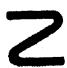
\includegraphics[keepaspectratio]{images/part002_3e3611b3.jpg}}

Remark 2. In a uniform space X a relatively compact set A is precompact, since A is contained in a compact set. On the other hand, even if X is Hausdorff, a precompact set need not be relatively compact in X, as is shown by the case where X itself is precompact but not compact.

PROPOSITION 2. Let \(f: \mathbf{X} \to \mathbf{Y}\) be a uniformly continuous mapping. If \(\mathbf{A}\) is any precompact subset of \(\mathbf{X}\) , then \(f(\mathbf{A})\) is a precompact subset of \(\mathbf{Y}\) . For if \(i: \mathbf{X} \to \hat{\mathbf{X}}\) and \(j: \mathbf{Y} \to \hat{\mathbf{Y}}\) are the canonical mappings, we have \(j(f(\mathbf{A})) = \hat{f}(i(\mathbf{A}))\) (§ 3, no. 7, Proposition 15) and hence \(j(f(\mathbf{A}))\) is relatively compact in \(\hat{\mathbf{Y}}\) (Chapter I, § 9, no. 4, Theorem 2, Corollary 1).

PROPOSITION 3. Let X be a set, let \((\mathrm{Y}_{\lambda})_{\lambda \in \mathbf{L}}\) be a family of uniform spaces, and for each \(\lambda \in L\) let \(f_{\lambda}\) be a mapping of X into \(Y_{\lambda}\) . Let X carry the coarsest uniformity for which the \(f_{\lambda}\) are uniformly continuous. Then a subset A of X is precompact if and only if \(f_{\lambda}(A)\) is a precompact subset of \(Y_{\lambda}\) for each \(\lambda \in L\) .

The condition is necessary by virtue of Proposition 2. Sufficiency follows from the characterization of the Hausdorff completion of X given in § 3, no. 9, Proposition 18, and Tychonoff's theorem (Chapter I, § 9, Theorem 3, Corollary).

\subsection{COMPACT SETS IN A UNIFORM SPACE}

The following proposition for an arbitrary uniform space is a sharper form of Proposition 2 of Chapter I, § 9, no. 2 for compact spaces.

PROPOSITION 4. In a uniform space X, let A be a compact set and B a closed set such that A∩B=∅. Then there is an entourage V of X such that V(A) and V(B) do not intersect.

If the proposition were false, then none of the sets \(A \cap \mathring{V}(B)\) , where V runs through the set of symmetric entourages of X, would be empty; hence these sets would form a filter base on A, which would have a cluster point \(x_0 \in A\) . Hence for each symmetric entourage \(V\) of \(X\) , \(\dot{V}(x_0)\) would meet \(B\) and therefore, as \(B\) is closed, we should have \(x_0 \in B\) , contrary to hypothesis.

COROLLARY. Let A be a compact set in a uniform space X; then as V runs through the set of entourages of X, the sets V(A) form a fundamental system of neighbourhoods of A.

Let U be any open neighbourhood of A, then B = CU is closed and does not meet A; hence, by Proposition 4, there is an entourage V such that \(\mathrm{V}(\mathrm{A}) \cap \mathrm{V}(\mathrm{B}) = \varnothing\) , and therefore \(\mathrm{V}(\mathrm{A}) \subset \mathrm{U}\) .

\subsection{CONNECTED SETS IN A COMPACT SPACE}

DEFINITION 3. Let V be a symmetric entourage of a uniform space X. A finite sequence \((x_{i})_{0\leqslant i\leqslant n}\) of points of X is said to be a V-chain if \(x_{i}\) and \(x_{i+1}\) are V-close for \(0\leqslant i<n\) . The points \(x_{0}\) and \(x_{n}\) are called the ends of the V-chain, and they are said to be joined by the V-chain.

Given a symmetric entourage V, the relation ``there is a V-chain joining x and y'' is an equivalence relation between x and y in X. Let \(A_{x,v}\) be the equivalence class of x for this relation, i.e.~the set of all \(y \in X\) which can be joined to x by a V-chain. Clearly if \(y \in A_{x,v}\) then \(\mathrm{V}(y) \subset \mathrm{A}_{x,\mathrm{v}}\) ; hence \(A_{x,v}\) is open in X; and the complement of \(A_{x,v}\) , being a union of equivalence classes, is also open. Hence:

PROPOSITION 5. In a uniform space X, the set \(A_{x,v}\) of points which can be joined by a V-chain to a given point x is both open and closed in X.

For each \(x \in X\) , let \(A_{x}\) denote the intersection of the sets \(A_{x,v}\) as V runs through the set of symmetric entourages of X; \(A_{x}\) is the equivalence class of x for the equivalence relation ``for all symmetric entourages V, there is a V-chain joining x and y''.

PROPOSITION 6. In a compact space X, the component of x, the set \(A_{x}\) , and the intersection of the neighbourhoods of x which are both open and closed, are all three identical.

It is enough to show that \(A_{x}\) is connected: for in any uniform space X the component of x is contained in the intersection of the neighbourhoods of x which are both open and closed, and this intersection is contained in \(A_{x}\) by Proposition 5.

Suppose \(A_{x}\) is not connected. Since \(A_{x}\) is closed, there are two non-empty disjoint closed sets B and C such that \(B \cup C = A_{x}\) . By Proposition 4 of §3 there is an entourage U of X such that \(U(B) \cap U(C)\) is empty.

Let W be an open entourage such that \(\hat{W} \subset U\) , and let H be the closed set which is the complement of \(W(B) \cup W(C)\) in X. Suppose for example that \(x \in B\) , and let y be a point of C. Then for each symmetric entourage \(V \subset W\) one sees immediately, by induction on i, that every V-chain \((x_{i})_{0 \leqslant i \leqslant n}\) joining x and y in X must have a point in H, by the choice of W. Since by hypothesis x and y can be joined by a V-chain for each symmetric entourage V, we see that \(H \cap A_{x,v}\) is not empty if \(V \subset W\) . On the other hand, if \(V' \subset V\) then clearly \(A_{x,v'} \subset A_{x,v}\) ; thus it follows that, as V runs through the set of symmetric entourages of X, the sets \(H \cap A_{x,v}\) form a filter base of closed sets in the compact space H. Hence all these sets have a common point and therefore H meets \(A_{x}\) ; but this contradicts the definition of H.

COROLLARY. Let X be a locally compact space and let K be a compact component of X. Then the neighbourhoods of K which are both open and closed form a fundamental system of neighbourhoods of K.

Let V be a relatively compact open neighbourhood of K in X (Chapter I, § 9, no. 7, Proposition 10) and let F be its frontier. Let U ⊂ V be a set which is both open and closed with respect to V. Then U is closed in X, and if in addition U does not meet F, then U is open in X (for then U ⊂ V and U is open in V). Hence it is enough to show that there is a subset of V which contains K, does not meet F and is both open and closed with respect to V.

Suppose this is not the case: then the intersections of F with the subsets of \(\overline{V}\) which contain K and are open and closed in \(\overline{V}\) form a filter base of closed sets in F; F is compact, so these sets have a common point \(y \in F\) . But this is absurd; since \(\overline{V}\) is compact, K is a component of \(\overline{V}\) , and by virtue of Proposition 6, the intersection of the sets which contain K and are both open and closed in \(\overline{V}\) is just K. The Corollary is thus proved.

PROPOSITION 7. Let X be a compact space and let R be the equivalence relation on X whose classes are the components of X. Then the quotient space X/R is compact and totally disconnected.

We know from Chapter I, § II, no. 5, Proposition 9 that X/R is totally disconnected; hence we have to show that X/R is Hausdorff (Chapter I, § 10, no. 4, Proposition 8.) Let A and B be two distinct components of X. By Proposition 6 there is a symmetric entourage U of X such that no point of A can be joined to any point of B by a U-chain. The set V (resp. W) of points of X which can be joined to a point \(x \in A\) (resp. \(y \in B\) ) by a U-chain is both open and closed in X (Proposition 5) and contains A (resp. B); these sets are therefore open neighbourhoods of A and B respectively, are saturated with respect to R and do not intersect. This completes the proof.

\BourbakiExercises

\BourbakiExerciseGroup

\begin{enumerate}
\def\labelenumi{\arabic{enumi})}
\tightlist
\item
  Let X be an infinite set and let F be an ultrafilter on X such that the sets of F have empty intersection. For each \(A \in F\) , let \(V_{A}\) denote the subset \(\Delta \cup (A \times A)\) of \(X \times X\) . Show that, as A runs through F, the sets \(V_{A}\) form a fundamental system of entourages for a uniformity \(\mathcal{U}(\mathfrak{F})\) on X, and that the topology induced by this uniformity is discrete.
\end{enumerate}

*2) On the real line R, carrying the additive uniformity, show that as V runs through the filter of entourages of R the sets V(Z) do not form a fundamental system of neighbourhoods of the set Z of rational integers.* (Cf. § 4, no. 3, Corollary to Proposition 4).

*3) Let V be that entourage of the additive uniformity on R which consists of all pairs \((x, y)\) such that either \(|x - y| \leqslant 1\) or \(xy \geqslant 1\) . Show that V is closed in \(R \times R\) , but that if A denotes the (closed) subset of R consisting of all integers \(n \geqslant 2\) , then \(V(A)\) is not closed in \(R\).*

\begin{enumerate}
\def\labelenumi{\arabic{enumi})}
\setcounter{enumi}{3}
\tightlist
\item
  Show that if a uniform space is a Kolmogoroff space (Chapter I, § 1, Exercise 2) then it is Hausdorff.
\end{enumerate}

¶ 5) a) Let X be a uniform space, U its uniformity; for each entourage V of X, let \(\tilde{V}\) be the subset of \(\mathfrak{P}(X) \times \mathfrak{P}(X)\) consisting of all pairs (M, N) of subsets of X such that both \(M \subset V(N)\) and \(N \subset V(M)\) . Show that the sets \(\tilde{V}\) form a fundamental system of entourages of a uniformity \(\tilde{U}\) on \(\mathfrak{P}(X)\) .

\begin{enumerate}
\def\labelenumi{\alph{enumi})}
\setcounter{enumi}{1}
\item
  On the set \(\mathfrak{P}_{0}(\mathbf{X})\) of non-empty subsets of \(\mathbf{X}\) , show that the topology induced by the topology \(\mathfrak{C}(\tilde{\mathcal{U}})\) induced by \(\tilde{\mathcal{U}}\) is finer than the topology \(\mathfrak{C}_{\Phi}\) (Chapter I, § 2, Exercise 7).
\item
  If X has at least two points and if U is Hausdorff, show that the topology induced by \(\mathfrak{G}(\tilde{\mathcal{U}})\) on \(\mathfrak{P}_{0}(\mathbf{X})\) is never coarser than \(G_{\Omega}\) . The topology induced by \(\mathfrak{G}(\tilde{\mathcal{U}})\) on the set \(\mathfrak{F}(\mathbf{X})\) of non-empty closed subsets of X is finer than the topology induced by \(G_{\Omega}\) on this set if and only if, for each closed subset A of X, the sets V(A) form a fundamental system of neighbourhoods of A as V runs through the set of entourages of X.
\end{enumerate}

*d) Show that on the quotient set X/R defined in Chapter I, § 11, Exercise 18, the quotient topology, and the topologies defined by \(\mathfrak{C}_{\Omega}\) , \(\mathfrak{C}_{\Phi}\) and \(\mathfrak{C}(\tilde{\mathcal{U}})\) (where \(\mathcal{U}\) is the usual uniformity on \(\mathbf{R}^2\) ) are all four distinct.*

\BourbakiExerciseGroup

\(^{*}\) 1) Show that on the real line R (with the additive uniformity) the function \(|x|\) is uniformly continuous; the function \(1/x\) is uniformly continuous in every interval \([a, +\infty[\) where a \textgreater{} 0; and that this function is continuous, but not uniformly continuous, in the interval \(]0, +\infty[\cdot*\)

\begin{enumerate}
\def\labelenumi{\arabic{enumi})}
\setcounter{enumi}{1}
\item
  Show that the topologies induced on Z by the p-adic uniformities are not comparable for different primes p.
\item
  Let \(\mathfrak{F}_1, \mathfrak{F}_2\) be two distinct ultrafilters on an infinite set X. Show that the uniformities \(\mathcal{U}(\mathfrak{F}_1)\) and \(\mathcal{U}(\mathfrak{F}_2)\) ( \(\S\) I, Exercise I) are not comparable, and that their least upper bound is the discrete uniformity. What is their greatest lower bound? Deduce that the set of Hausdorff uniformities on X is equipotent to \(\mathfrak{P}(\mathfrak{P}(X))\) {[}cf.~Chapter I, \(\S\) 8, Exercise 6 a){]}.
\item
  \begin{enumerate}
  \def\labelenumii{\alph{enumii})}
  \tightlist
  \item
    Let \(\mathfrak{U}\) and \(\mathfrak{U}'\) be the filters of entourages of two uniformities on the same non-empty set \(\mathbf{X}\) . Show that the intersection of the filters \(\mathfrak{U}\) and \(\mathfrak{U}'\) is the filter of entourages of a uniformity on \(\mathbf{X}\) if and only if, for each \(\mathbf{V} \in \mathfrak{U}\) and \(\mathbf{V}' \in \mathfrak{U}'\) , there exist \(\mathbf{W} \in \mathfrak{U}\) and \(\mathbf{W}' \in \mathfrak{U}'\) such that \(\mathbf{WW}' \subset \mathbf{V} \cup \mathbf{V}'\) .
  \end{enumerate}
\end{enumerate}

\begin{enumerate}
\def\labelenumi{\alph{enumi})}
\setcounter{enumi}{1}
\tightlist
\item
  Give an example of two filters of entourages \(\mathcal{U}_{\overline{\omega}}\) , \(\mathcal{U}_{\overline{\omega}'}\) , each defined by a finite partition of X (no. 5, Example), which do not satisfy the condition of \(a\) ).
\end{enumerate}

\begin{enumerate}
\def\labelenumi{\arabic{enumi})}
\setcounter{enumi}{4}
\tightlist
\item
  Let \((\mathbf{X}_i)_{i\in I}\) be a family of uniform spaces and let \(c\) be an infinite cardinal. For each family \((\mathbf{V}_i)_{i\in H}\) , where card \((\mathbf{H}) < c\) and \(\mathbf{V}_i\) is an entourage of \(\mathbf{X}_i\) for each \(i\in H\) , let \(\mathbf{U}((\mathbf{V}_i))\) be the set of pairs \((x,y)\) of points of \(\mathbf{X} = \prod_{i \in I}\mathbf{X}_i\) such that \((\mathrm{pr}_i x, \mathrm{pr}_i y) \in \mathbf{V}_i\) for each \(i\in H\) .
\end{enumerate}

Show that the sets \(\mathbf{U}((\mathbf{V}_{i}))\) form a fundamental system of entourages of a uniformity on X, and that the topology induced by this uniformity is that defined in Exercise 9 of Chapter I, § 4.

\begin{enumerate}
\def\labelenumi{\arabic{enumi})}
\setcounter{enumi}{5}
\tightlist
\item
  Let X be a uniform space, U its uniformity, \(\tilde{U}\) the corresponding uniformity on \(\mathfrak{P}(X)\) (§ 1, Exercise 5).
\end{enumerate}

\begin{enumerate}
\def\labelenumi{\alph{enumi})}
\item
  Show that the mapping \(x \to \{x\}\) is an isomorphism of the uniform space \(X\) onto a subspace of the uniform space \(\mathfrak{P}(X)\) .
\item
  Show that the uniformity induced by \(\widetilde{\mathcal{U}}\) on the set \(\mathfrak{F}(\mathbf{X})\) of non-empty closed subsets of \(\mathbf{X}\) is Hausdorff, and that \(\widetilde{\mathcal{U}}\) is the inverse image under the mapping \(\mathbf{M} \to \overline{\mathbf{M}}\) of the uniformity induced by \(\widetilde{\mathcal{U}}\) on \(\mathfrak{F}(\mathbf{X})\) . c) Show that the mapping \((\mathbf{M}, \mathbf{N}) \to \mathbf{M} \cup \mathbf{N}\) of \(\mathfrak{P}(\mathbf{X}) \times \mathfrak{P}(\mathbf{X})\) into \(\mathfrak{P}(\mathbf{X})\) is uniformly continuous.
\item
  Let Y be another uniform space. If \(f: X \to Y\) is a uniformly continuous mapping, show that the mapping \(M \to f(M)\) of \(\mathfrak{P}(X)\) into \(\mathfrak{P}(Y)\) is uniformly continuous.
\item
  Let \(\mathfrak{M}\) be a compact subset of the set \(\mathfrak{F}(\mathbf{X})\) of non-empty closed subsets of \(\mathbf{X}\) , \(\mathfrak{F}(\mathbf{X})\) carrying the topology induced by the topology \(\mathfrak{C}(\tilde{\mathcal{U}})\) induced by \(\tilde{\mathcal{U}}\) . Show that the set \(\bigcup_{\mathbf{M} \in \mathfrak{M}} \mathbf{M}\) is closed in \(\mathbf{X}\) .
\end{enumerate}

\BourbakiExerciseGroup

\(^{*1}\) Let U denote the additive uniformity on the real line R, and let \(U'\) denote the inverse image of U under the mapping \(x \rightarrow x^{3}\) of R onto itself. Show that \(U'\) is strictly finer than U, but that the Cauchy filters are the same for both uniformities. \(^{*}\)

\begin{enumerate}
\def\labelenumi{\arabic{enumi})}
\setcounter{enumi}{1}
\tightlist
\item
  \begin{enumerate}
  \def\labelenumii{\alph{enumii})}
  \tightlist
  \item
    Let X be an infinite set and let F be a non-trivial ultrafilter on X. Show that if X carries the uniformity \(\mathcal{U}(\mathfrak{F})\) (§ 1, Exercise 1) then the complement of X in its completion \(\hat{X}\) consists of a single point, and that the topological space \(\hat{X}\) can be identified with the space associated with the ultrafilter F (Chapter I, § 6, no. 5, Example).
  \end{enumerate}
\end{enumerate}

*b) Deduce from a) an example of a uniformity on R which is finer than the additive uniformity and with respect to which R is not complete.*

*3) a) Let \(\mathcal{U}\) denote the additive uniformity on the real line \(\mathbf{R}\) , let \(\mathcal{U}_1\) denote the uniformity induced on \(\mathbf{R}\) by that of the extended line \(\overline{\mathbf{R}}\) , and let \(\mathcal{U}_2\) denote the uniformity induced on \(\mathbf{R}\) by that of the one-point compactification \(\tilde{\mathbf{R}} = \mathbf{P}_1(\mathbf{R})\) of \(\mathbf{R}\) . Show that \(\mathcal{U}\) is strictly finer than \(\mathcal{U}_1\) , that \(\mathcal{U}_1\) is strictly finer than \(\mathcal{U}_2\) , and that the topologies induced by these three uniformities are the same; also that the completions of \(\mathbf{R}\) with respect to these three uniformities are respectively \(\mathbf{R}\) , \(\overline{\mathbf{R}}\) and \(\tilde{R}\) . The identity mapping of R extends by continuity to an injective but not surjective mapping \(R \rightarrow \overline{R}\) and to a surjective but not injective mapping \(\overline{R} \rightarrow \tilde{R}\) .

\begin{enumerate}
\def\labelenumi{\alph{enumi})}
\setcounter{enumi}{1}
\tightlist
\item
  Deduce from a) an example of two Hausdorff uniform spaces X, Y and a uniformly continuous bijection \(u: X \rightarrow Y\) whose extension by continuity \(\overline{u}: \hat{X} \rightarrow \hat{Y}\) is neither injective nor surjective.*
\end{enumerate}

¶ 4) With the notation of Exercise 5 of § 2, suppose that all the uniform spaces \(X_i\) are complete. Show that the space \(X\) is complete with respect to the uniformity there defined (argue by reductio ad absurdum, using § 2, Proposition 5, Corollary 2).

\begin{enumerate}
\def\labelenumi{\arabic{enumi})}
\setcounter{enumi}{4}
\item
  Let X be a Hausdorff uniform space such that X is the intersection of a countable family of open sets of \(\hat{X}\) . Show that if Y is any Hausdorff uniform space which contains X as a uniform subspace, then X is the intersection of a closed subset of Y and a countable family of open sets of Y.
\item
  Let X be a uniform space and let \(i: X \to \hat{X}\) be the canonical mapping of X into its Hausdorff completion. Let \(X_{0}\) be the sum of X and \(\hat{X} - i(X)\) , and let \(j: X_{0} \to \hat{X}\) be the mapping which agrees with i on X and with the identity mapping on \(\hat{X} - i(X)\) . Show that \(X_{0}\) is complete with respect to the uniformity which is the inverse image under j of the uniformity of \(\hat{X}\) , also that if Y is any complete uniform space such that X is a uniform subspace of Y, then the identity mapping \(X \to X\) can be extended uniquely to a continuous mapping \(X_{0} \to Y\) .
\end{enumerate}

¶ 7) Let \(\mathbf{X}\) be a Hausdorff uniform space, \(\mathcal{U}\) its uniformity, \(\mathcal{U}_0\) the uniformity induced on \(\mathfrak{F}(\mathbf{X})\) by the uniformity \(\tilde{\mathcal{U}}\) ( \(\S\) 2, Exercise 6 b), \(\mathcal{U}_{00}\) the uniformity induced on \(\mathfrak{F}(\mathfrak{F}(\mathbf{X}))\) by the uniformity \(\tilde{\mathcal{U}}_0\) . Show that the canonical mapping \(x \to \{\{x\}\}\) of \(\mathbf{X}\) into \(\mathfrak{F}(\mathfrak{F}(\mathbf{X}))\) extends to an isomorphism of \(\hat{\mathbf{X}}\) onto a closed uniform subspace of \(\mathfrak{F}(\mathfrak{F}(\mathbf{X}))\) (carrying the uniformity \(\mathcal{U}_{00}\) ) (use Proposition 9 of no. 4).

\BourbakiExerciseGroup

¶ 1) Let R be an open covering of a compact space X. Show that there is an entourage V of the uniformity of X such that, for each \(x \in X\) , \(V(x)\) is contained in a set belonging to R {[}remark that for each \(x \in X\) there is an entourage \(W_x\) such that \(\dot{W}_x(x)\) is contained in a set of R, and cover X by a finite number of sets \(W_x(x)\) {]}.

\begin{enumerate}
\def\labelenumi{\arabic{enumi})}
\setcounter{enumi}{1}
\item
  Prove that a quasi-compact space X is uniformizable if and only if its topology is the inverse image of the topology of a compact space Y under a surjective mapping \(f: X \rightarrow Y\) .
\item
  Let \(f\) be a continuous mapping of a compact space \(\mathbf{X}\) into a compact space \(\mathbf{Y}\) , and let \(\mathbf{V}\) be an open entourage of \(\mathbf{X}\) such that the relation \(f(x) = f(y)\) implies \((x, y) \in \mathbf{V}\) . Show that there is an entourage \(W\) of \(\mathbf{Y}\) such that the relation \((f(x), f(y)) \in W\) implies \((x, y) \in V\) .
\item
  Let X be the locally compact space defined in Chapter I, § 9, Exercise II. Show that every neighbourhood of the diagonal \(\Delta\) in \(X \times X\) contains a set of the form \([x, b[ \times [x, b[\) . Deduce that there is only one uniformity on X compatible with the topology of X, and that the completion of X for this uniformity can be identified with the interval \(X' = [a, b]\) carrying the topology \(\mathcal{C}v(X)\) . (Observe that every ultrafilter on X must be a Cauchy filter with respect to any uniformity compatible with the topology of X).
\item
  Show that a uniform space X is precompact if and only if every ultrafilter on X is a Cauchy filter. (Remark that if X is not precompact then there is an entourage V of X such that the sets \(\mathbb{C}\mathrm{V}(x)\) , as x runs through X, generate a filter on X).
\item
  Let X be a uniform space in which every sequence of points has at least one cluster point. Show that X is precompact (use reductio ad absurdum).
\item
  A subset \(\mathbf{A}\) of a uniform space \(\mathbf{X}\) is said to be bounded if for each entourage \(\mathbf{V}\) of \(\mathbf{X}\) there is a finite set \(\mathbf{F}\) and an integer \(n > 0\) such that \(\mathbf{A} \subset \overset{n}{\mathbf{V}}(\mathbf{F})\) .
\end{enumerate}

\begin{enumerate}
\def\labelenumi{\alph{enumi})}
\item
  The union of two bounded subsets is bounded. The closure of a bounded subset is bounded. Every precompact subset is bounded.
\item
  If \(f: \mathbf{X} \to \mathbf{Y}\) is uniformly continuous, then the image under \(f\) of every bounded subset of \(\mathbf{X}\) is a bounded subset of \(\mathbf{Y}\) .
\item
  In a product of non-empty uniform spaces, a set is bounded if and only if each of its projections is bounded.
\item
  For each symmetric entourage V of X, let \(R_{V}\) denote the union of the sets \(\stackrel{n}{V}\) as n runs through the integers \textgreater0. Show that \(R_{V}\) is both open and closed in \(X \times X\) and that, in the notation of no. 4,
\end{enumerate}

\[
\mathbf {R} _ {\mathbf {v}} (x) = \mathbf {A} _ {x, \mathbf {v}}
\]

for each \(x \in \mathbf{X}\) . Suppose that \(\mathbf{R}_{\mathbf{V}} = \mathbf{X} \times \mathbf{X}\) for each symmetric entourage \(\mathbf{V}\) of \(\mathbf{X}\) (this will be the case in particular if \(\mathbf{X}\) is connected); show that a set \(\mathbf{A} \subset \mathbf{X}\) is bounded if and only if, for each symmetric entourage \(\mathbf{V}\) of \(\mathbf{X}\) and each \(x_0 \in \mathbf{X}\) , there is an integer \(n > 0\) such that \(\mathbf{A} \subset \mathbf{V}(x_0)\) .

\begin{enumerate}
\def\labelenumi{\arabic{enumi})}
\setcounter{enumi}{7}
\item
  Let X be a uniform space, V a closed entourage of X, A a compact subset of X. Show that V(A) is closed in X (cf.~Chapter I, § 10, no. 2, Theorem 1, Corollary 5).
\item
  Let X be a locally compact space which carries a uniformity compatible with its topology and is such that there is an entourage V with the property that \(V(x)\) is relatively compact in X for all \(x \in X\) . a) Show that X is complete with respect to this uniformity.
\end{enumerate}

\begin{enumerate}
\def\labelenumi{\alph{enumi})}
\setcounter{enumi}{1}
\item
  Let \(\mathbf{U}\) be a symmetric entourage of \(\mathbf{X}\) such that \(\dot{\mathbf{U}}\subset\mathbf{V}\) . Show that if \(\mathbf{A}\) is relatively compact in \(\mathbf{X}\) , then so is \(\mathbf{U}(\mathbf{A})\) .
\item
  Show that X is paracompact {[}use b), Exercise 7 and Chapter I, § 9, no. 10, Theorem 5{]}.
\item
  Let W be a closed symmetric entourage of X such that \(\dot{W} \subset V\) . Show that if A is closed in X then so is \(\mathbf{W}(\mathbf{A})\) (use Exercise 8).
\end{enumerate}

\begin{enumerate}
\def\labelenumi{\arabic{enumi})}
\setcounter{enumi}{9}
\tightlist
\item
  Let X be a Hausdorff uniform space which has an entourage V such that \(\mathbf{V}(x)\) is precompact for each \(x \in X\) . Show that the completion \(\hat{X}\) is locally compact and satisfies the conditions of Exercise 9. {[}If W is a symmetric open entourage of X such that \(\hat{W} \subset V\) , show that the closure \(\overline{W}\) of W in \(\hat{X} \times \hat{X}\) is such that \(\overline{W}(x)\) is compact for each \(x \in \hat{X}\) {]}.
\end{enumerate}

¶ 11) Let X be a Hausdorff uniform space, U its uniformity, F(X) the set of all non-empty closed subsets of X. Let F(X) carry the uniformity induced by the uniformity U defined in § 1, Exercise 5 a).

\begin{enumerate}
\def\labelenumi{\alph{enumi})}
\item
  Show that if \(X'\) is precompact then so is \(\mathfrak{F}(\mathbf{X})\) . {[}If \((\mathbf{A}_{i})\) is a finite covering of X by V-small sets (V symmetric), show that the sets \(\tilde{\mathbf{V}}(\mathbf{B}_{k})\) cover \(\mathfrak{F}(\mathbf{X})\) , where the \(B_{k}\) are all the unions of sets \(A_{i}]\) .
\item
  A point \(\mathbf{A} \in \mathfrak{F}(\mathbf{X})\) is such that every neighbourhood of \(\mathbf{A}\) in the topology induced by \(\mathfrak{G}(\tilde{\mathcal{U}})\) on \(\mathfrak{F}(\mathbf{X})\) contains a neighbourhood of \(\mathbf{A}\) in the topology induced by \(\mathfrak{G}_{\Theta}\) (Chapter I, § 8, Exercise 12) on \(\mathfrak{F}(\mathbf{X})\) , if and only if \(\mathbf{A}\) is precompact.
\item
  Show that the topologies \(\mathfrak{G}(\mathfrak{U})\) and \(\mathfrak{G}_{\Theta}\) induce the same topology on the set \(\mathfrak{K}(\mathbf{X})\) of compact subsets of \(\mathbf{X}\) {[}use \(b\) ) and Exercise 5 of §1{]}.
\end{enumerate}

\begin{enumerate}
\def\labelenumi{\arabic{enumi})}
\setcounter{enumi}{11}
\tightlist
\item
  \begin{enumerate}
  \def\labelenumii{\alph{enumii})}
  \tightlist
  \item
    Let R be a Boolean algebra, and identify R with a Boolean algebra of subsets of the set \(\Omega\) of maximal prefilters on R (Chapter I, § 6, Exercise 20). For each finite partition \(\overline{\omega} = (\mathbf{A}_i)\) of \(\Omega\) , formed of sets belonging to R, let \(\mathbf{C}_{\overline{\omega}}\) denote the subset \(\bigcup_{i} (\mathbf{A}_i \times \mathbf{A}_i)\) of \(\Omega \times \Omega\) .
  \end{enumerate}
\end{enumerate}

Show that the sets \(C_{\overline{\omega}}\) form a fundamental system of entourages of a Hausdorff uniformity on \(\Omega\) . The completion, \(\hat{\Omega}\) , of \(\Omega\) with respect to this uniformity is a totally disconnected compact space. A subset of \(\hat{\Omega}\) is both open and closed in \(\hat{\Omega}\) if and only if it is of the form \(\overline{\mathbf{A}}\) , where \(\mathbf{A} \in \mathbf{R}\) . Show that \(\mathbf{A} \to \overline{\mathbf{A}}\) is a bijective mapping of \(\mathbf{R}\) onto the set of subsets of \(\hat{\Omega}\) which are both open and closed, and that \(\overline{\mathbf{C}}\mathbf{A} = \overline{\mathbf{C}}\overline{\mathbf{A}}\) , \(\overline{\mathbf{A} \cup \mathbf{B}} = \overline{\mathbf{A}} \cup \overline{\mathbf{B}}\) and \(\overline{\mathbf{A} \cap \mathbf{B}} = \overline{\mathbf{A}} \cap \overline{\mathbf{B}}\) . Deduce that the canonical mapping \(\Omega \to \hat{\Omega}\) is bijective.

\begin{enumerate}
\def\labelenumi{\alph{enumi})}
\setcounter{enumi}{1}
\tightlist
\item
  Let X be a Hausdorff topological space in which the sets that are both open and closed form a base for the topology. Take R to be the Boolean algebra formed by subsets of X which are both open and closed; then the topology induced on X by the topology of the completion \(\hat{\mathbf{X}}\) of X with respect to the uniformity \(\mathcal{U}\) defined in \(a\) ) is the given topology on X. Further, the maximal elements of the set of filters on X having a base formed of open sets, and the maximal elements of the set of filters on X having a base formed of closed sets are Cauchy filters with respect to the uniformity \(\mathcal{U}\) . Deduce that there are continuous surjections \(\varphi: \hat{\mathbf{X}} \to \hat{\mathbf{X}}, \psi: \mathbf{X}' \to \hat{\mathbf{X}}\) , where \(\hat{\mathbf{X}}, \mathbf{X}'\) are the spaces defined in Chapter I, § 9, Exercises 25 and 24. * Show that if X is the rational line Q, then \(\psi\) is not bijective.* If X is extremally disconnected (Chapter I, § 11, Exercise 21), then \(\psi\) is bijective, \(\hat{\mathbf{X}}\) is extremally disconnected and can be identified with the semi-regular space associated with \(\mathbf{X}'\) (Chapter I, § 8, Exercise 20); thus extremally disconnected spaces can be characterized as dense subspaces of extremally disconnected compact spaces. Hence give an example of an extremally disconnected compact space which has no isolated points {[}(cf.~Chapter I, § 11, Exercise 21 f){]}.
\end{enumerate}

In particular, if we take X to be a discrete space, then \(\hat{X}\) can be identified with the ultrafilter space of X (Chapter I, § 9, Exercise 26).

13) Let X be a locally compact space and U an open subset of X. Let B be the union of U and the relatively compact components of CU. Show that B is open and is the union of U and those subsets of CU which are both open and compact in CU. (Embed X in its one-point compactification \(X' = X \cup \{\omega\}\) , observe that in \(X' - U\) the component of \(\omega\) is \(\{\omega\} \cup CB\) , and use Proposition 6 of no. 4).

\begin{enumerate}
\def\labelenumi{\arabic{enumi})}
\setcounter{enumi}{13}
\item
  Let X be a compact space, and let B be a filter base on X consisting of connected closed sets. Show that the (non-empty) intersection of the sets of B is closed and connected (argue by reductio ad absurdum, using Proposition 4 of no. 3 and Chapter I, § 9, no. 1, Theorem 1).
\item
  Let X be a compact space. Then the space \(\mathfrak{F}(\mathbf{X})\) of non-empty closed subsets of X, with the topology induced by \(\mathcal{C}(\tilde{\mathcal{U}})\) (Exercise 11), is compact (Chapter I, § 9, Exercise 13). Consider an ultrafilter \(\Psi\) on \(\mathfrak{F}(\mathbf{X})\) , and suppose that for each entourage V of the uniformity of X, and each \(\mathfrak{X} \in \Psi\) , there exists \(\mathbf{M} \in \mathfrak{X}\) such that any two points of \(\mathbf{M}\) can be joined by a V-chain contained in \(\mathbf{M}\) . Show that the limit point A of \(\Psi\) in \(\mathfrak{F}(\mathbf{X})\) is a connected subset of \(\mathbf{X}\) (use Proposition 6 of no. 4).
\item
  Let X be a connected compact space and let A, B be two disjoint non-empty closed subsets of X. Show that there is a component of \(\mathbb{C}(\mathrm{A} \cup \mathrm{B})\) whose closure meets both A and B. (Let U be an entourage of the uniformity of X such that \(\overline{\mathbf{U}}(\mathbf{A}) \cap \overline{\mathbf{U}}(\mathbf{B}) = \varnothing\) . Show first that the set \(\mathfrak{M}_{\mathrm{U}}\) of components of \(\overline{\mathbb{C}(\mathrm{U}(\mathbf{A}) \cup \mathrm{U}(\mathbf{B}))}\) which meet both \(\overline{\mathrm{U}(\mathbf{A})}\) and \(\overline{\mathrm{U}(\overline{\mathrm{B}})}\) is not empty, by proving that for each symmetric entourage W ⊂ U there exist \(x \in \mathrm{U}(\mathbf{A})\) and \(y \in \mathrm{U}(\mathbf{B})\) and a W-chain which joins x to y and all of whose points other than x and y belong to \(\mathbb{C}(\mathrm{U}(\mathbf{A}) \cup \mathrm{U}(\mathbf{B}))\) , and then applying Exercise 15. For each entourage V ⊂ U, show that every K ∈ \(\mathfrak{M}_{\mathrm{V}}\) contains a set H ∈ \(\mathfrak{M}_{\mathrm{U}}\) , and that the set \(\mathfrak{M}_{\mathrm{U},\mathrm{V}}\) of sets H ∈ \(\mathfrak{M}_{\mathrm{U}}\) which are contained in a set K ∈ \(\mathfrak{M}_{\mathrm{V}}\) is closed in \(\mathfrak{F}(\overline{\mathrm{X}})\) ; and conclude that as V runs through the set of entourages contained in U, the intersection of the sets \(\mathfrak{M}_{\mathrm{U},\mathrm{V}}\) is not empty).
\item
  Let X be a connected locally compact space. Let K be any non-empty compact subset of X distinct from X. Show that every component of K meets the frontier of K in X (use the Corollary to Proposition 6 of no. 4). Deduce that if A is any non-empty relatively compact open subset of X distinct from X, then the closure of every component of A meets CA.
\end{enumerate}

¶ 18) a) Show that a compact connected space X cannot be the union of a countable infinity of mutually disjoint non-empty closed sets {[}by reductio ad absurdum: if (F \(_{n}\) ) is a countably infinite partition of X into closed sets, show with the help of Exercise 17 that there is a compact connected set K which does not meet F \(_{1}\) but meets an infinite number of sets F \(_{n}\) ; in order to do this consider the component of a point of F \(_{2}\) with respect to a compact neighbourhood of F \(_{2}\) not meeting F \(_{1}\) . Then use induction{]}.

\begin{enumerate}
\def\labelenumi{\alph{enumi})}
\setcounter{enumi}{1}
\tightlist
\item
  Extend the result of a) to a locally compact connected space X under one or the other of the following two supplementary conditions: one of the \(F_{n}\) is compact and connected, or X is locally connected. {[}In the first case, reduce to a) by means of Exercise 17{]}.
\end{enumerate}

\(^{*}c)\) Let \(\mathbf{X}\) be the subspace of \(\mathbb{R}^3\) which is the union of the following subspaces: \(A_n\) is the half-line \(x > 0\) , \(y = 1/n\) , \(z = 0\) ( \(n \geqslant 1\) ); \(B_n\) is the interval \(2n < x < 2n + 2\) , \(y = 0\) , \(z = 0\) ( \(n \geqslant 0\) ); \(C_n\) is the set defined by the relations

\[
x = 2 n + 1, \quad 0 \leqslant y \leqslant \frac {1}{n + 1}, \quad z = y \left(y - \frac {1}{n + 1}\right),
\]

where \(n \geqslant 0\) .

Show that X is connected and locally compact and is the union of a countable infinite family of mutually disjoint connected non-empty closed sets. *

¶ 19) A compact connected space X is said to be irreducible between two of its points x, y if there is no compact connected subset of X other than X itself which contains both x and y.

\begin{enumerate}
\def\labelenumi{\alph{enumi})}
\item
  If \(x\) and \(y\) are two distinct points of a compact connected space \(X\) , show that \(X\) has a compact connected subspace \(K\) which is irreducible between \(x\) and \(y\) (use Exercise 14 and Zorn's Lemma).
\item
  Show that a compact connected space having at least two points cannot be irreducible between every pair of its points (use Exercise 17).
\item
  Let X be a compact connected space, and suppose that there is a point \(a \in X\) which has a connected closed neighbourhood \(V \neq X\) . If x and y are any two points of CV, show that there is a compact connected subset of X which contains x and one of the points a, y but not the other (use Exercise 17). Under the same hypotheses, show that if x, y, z are any three distinct points of X, then X cannot be simultaneously irreducible between x and y, between y and z, and between x and z.
\end{enumerate}

\begin{enumerate}
\def\labelenumi{\arabic{enumi})}
\setcounter{enumi}{19}
\tightlist
\item
  Let X be a compact connected space and let L be the set of all points of X which have a fundamental system of connected neighbourhoods. The points of S = CL are called the singular points of X. The points of the interior \(\dot{L}\) of L and the components of \(\bar{S}\) are called the prime constituents of X.
\end{enumerate}

\begin{enumerate}
\def\labelenumi{\alph{enumi})}
\item
  Let \(\mathbf{A} \neq \mathbf{X}\) be a non-empty open subset of \(\mathbf{X}\) , let \(\mathbf{K}\) be a component of \(\overline{\mathbf{A}}\) and let \(\mathbf{F}\) be the closure of \(\overline{\mathbf{A}} \cap \mathbb{C}\mathbf{K}\) . Show that if \(\mathbf{A} \cap \mathbf{K} \cap \mathbf{F}\) is not empty then all its points are singular. If \(x \in \mathbf{A} \cap \mathbf{F} \cap \mathbf{K}\) , the component \(\mathbf{Q}\) of \(x\) in \(\mathbf{F}\) meets \(\mathbb{C}\mathbf{A}\) {[}consider a point of \(\mathbb{C}\mathbf{K}\) contained in \(V(x)\) and its component in \(\overline{\mathbf{A}}\) , and show by using Exercise 17 that the set of points of \(\mathbf{F}\) which can be joined to \(x\) by a V-chain in \(\mathbf{F}\) meets \(\mathbb{C}\mathbf{A}]\) . Deduce that the prime constituent \(\mathbf{P}\) which contains \(x\) meets \(\mathbb{C}\mathbf{A}\) (remark that \(\mathbf{P}\) contains the component of \(x\) in \(Q \cap A\) , and use Exercise 17 applied to the compact connected space \(Q\) and the open subset \(Q \cap A\) of \(Q\) ).
\item
  Deduce from a) that if P is a prime constituent of X and U is a neighbourhood of P, then P has a connected neighbourhood contained in U (by reductio ad absurdum).
\item
  Let V be a symmetric entourage of X, and let \(V'\) denote the set of pairs \((x, y)\) of points of X which can be joined by a V-chain, all of whose points are singular, except perhaps for x and y. As V runs through the symmetric entourages of X, the corresponding sets \(V'\) form a fundamental system of entourages of a uniformity (in general not Hausdorff) on X. Let \(X'\) be the associated Hausdorff space, and show that the inverse images of the points of \(X'\) under the canonical mapping \(X \rightarrow X'\) are the prime constituents of X. The (compact connected) space \(X'\) is called the space of prime constituents of X. Show that \(X'\) is locally connected {[}use b) and Chapter I, § 10, no. 4, Proposition 8{]}.
\end{enumerate}

\(^{*}d)\) Let \((r_{n})\) be the sequence of all the rational numbers contained in \(]0,1[\) , arranged in some order. For each irrational \(x\in[0,1]\) , let

\[
f (x) = \sum_ {n} 2 ^ {- n} \sin 1 / (x - r _ {n}).
\]

Let X be the closure in \(R^{2}\) of the graph of f.~Show that X is connected and irreducible between its points with abscissas 0 and 1, but that X has only one prime constituent.*

*21) In the locally compact space X defined in Exercise 20 b) of Chapter I, § 10, let S be the equivalence relation whose classes are the components of X. Show that the quotient space X/S is not Hausdorff.*

\begin{enumerate}
\def\labelenumi{\arabic{enumi})}
\setcounter{enumi}{21}
\tightlist
\item
  Show that every totally disconnected compact space X is homeomorphic to the inverse limit of an inverse system of finite discrete spaces. (Consider the finite partitions of X into open sets and use the Corollary to Proposition 6 of no. 4).
\end{enumerate}

¶ 23) Let \(f: \mathbf{X} \to \mathbf{Y}\) be a continuous open mapping, \(\mathbf{X}\) locally compact and \(\mathbf{Y}\) Hausdorff.

\begin{enumerate}
\def\labelenumi{\alph{enumi})}
\item
  If K is any compact connected subset of Y and C is any compact component of \(\overline{f}^{1}(K)\) , show that \(f(C)=K\) (reduce to the case K=Y and use the Corollary to Proposition 6 of no. 4). *Give an example of a non-compact component \(C'\) of \(\overline{f}^{1}(K)\) such that \(f(C')\neq K_*\)
\item
  Suppose in addition that Y is locally compact and locally connected. Show that if U is any connected open subset of Y and R is any relatively compact component of \(\overline{f}^{1}(U)\) in X, then \(f(R)=U\) . {[}Observe that in a locally compact locally connected space, a connected open set U is the union of the compact connected sets contained in U and containing a given point \(y_{0}\in U\) ; then apply a).{]}
\item
  Suppose in addition that X is locally connected. Show that if K is any connected subset of Y which is either open or compact with a non-empty interior, and if H is any compact subset of X, then there is only a finite number of components of \(\overline{f}^{1}(K)\) contained in H. {[}Use a) and b){]}.
\end{enumerate}

\BourbakiBackSection{HISTORICAL NOTE}

(Numbers in brackets refer to the bibliography at the end of this note.)

The principal concepts and results on uniform spaces have emerged gradually from the theory of real variables, and it is only in recent years that they have been systematically studied. Cauchy, in his attempt to put the theory of series on a rigorous basis (cf.~the Historical Notes to Chapters I and IV) took as starting point a principle which he seems to have thought self-evident, namely that a necessary and sufficient condition for the convergence of a sequence \((a_{n})\) is that \(|a_{n+p} - a_{n}|\) is as small as we please whenever n is sufficiently large (see for example {[}2{]}). Together with Bolzano {[}1{]} he was undoubtedly one of the first to state this principle explicitly and to recognize its importance; hence the name of ``Cauchy sequences'' given to sequences of real numbers which satisfy the condition in question, and by extension to sequences \((x_{n})\) of points in a metric space (Chapter IX) such that the distance from \(x_{n+p}\) to \(x_{n}\) is as small as we please whenever n is large enough; and hence finally the name of ``Cauchy filter'' given to the generalization of Cauchy sequences which has been studied in this chapter.

When later the intuitive notion of real number ceased to be regarded as adequate, and attempts were made to define real numbers in terms of rational numbers in order to provide a solid basis for Analysis, it was Cauchy's principle which provided the most fertile of the definitions put forward in the second half of the nineteenth century. This definition, due to Cantor {[}3{]} (and developed along the lines of Cantor's ideas by Heine {[}5{]} and independently by Méray, amongst others) consists in making a real number correspond to every Cauchy sequence of rational numbers (``fundamental sequence'' in Cantor's terminology); the same real number corresponds to two Cauchy sequences \((a_{n})\) and \((b_{n})\) of rational numbers if and only if \(|a_{n} - b_{n}|\) tends to zero. The essential idea here is that, from a certain point of view (in fact, the point of view of the ``uniform structure'' defined in this chapter, § 1, no. 1, Example 1), the set Q of rational numbers is ``incomplete'', and that the set of real numbers is the ``complete'' set which one gets from Q by ``completion''.

On the other hand, Heine was the first to define uniform continuity for real-valued functions of one or more real variables, in work largely inspired by the ideas of Weierstrass and Cantor {[}4{]}, and he proved that every real-valued function which is continuous on a bounded closed interval of R is uniformly continuous on this interval: this is ``Heine's theorem''. By Theorem 2 of § 4 this result is related to the compactness of a bounded closed interval of R (``Borel-Lebesgue theorem'', Chapter IV, § 2, Theorem 2; cf.~the Historical Notes to Chapters I and IV), and Heine's proof of his theorem can also serve, with some modifications, to prove the Borel-Lebesgue theorem (and this has appeared as sufficient reason to some authors for calling the latter theorem the ``Heine-Borel theorem'').

These ideas became extended to more general spaces when metric spaces came to be studied, first in particular cases and then in general (cf.~Chapter IX); in a metric space a distance is given (i.e.~a real-valued function of pairs of points, satisfying certain axioms) which defines both a topology and a uniformity. Fréchet, who was the first to give a general definition of these spaces, recognized the importance of Cauchy's principle {[}6{]} and also proved for metric spaces a theorem equivalent to Theorem 3 of § 4 ({[}6{]} and {[}7{]}). Hausdorff developed considerably the theory of metric spaces in his ``Mengenlehre'' ({[}8{]}; cf.~also {[}8 a{]}) and in particular realized that one can apply Cantor's construction, described earlier, to these spaces and hence obtain a ``complete'' metric space from a ``non-complete'' metric space (i.e.~one in which Cauchy's principle is not valid).

Metric spaces are a particular type of ``uniform spaces''; the latter were defined in full generality by A. Weil at a fairly recent date {[}9{]}. Previous to this, the notions and results on ``uniform structure'' could be used only in connection with metric spaces, and this fact explains the important part played by metric spaces and metrizable spaces (and in particular by compact metrizable spaces) in many modern works on topology, in questions where distance has no real usefulness. Once one has the definition of a uniform space, there is no difficulty (especially if one also has the notion of a filter at one's disposal) in extending to these spaces almost the whole of the theory of metric spaces as given e.g.~by Hausdorff (and similarly in extending, for example, to arbitrary compact spaces the results on compact metric spaces given in Alexandroff-Hopf's Topologie {[}10{]}). This is what we have done in this chapter; in particular, the theorem on completion of uniform spaces (§ 3, Theorem 3) is no more than a transposition, without any essential modifications, of Cantor's construction of the real numbers.

\BourbakiBackSection{BIBLIOGRAPHY}

{[}1{]} B. BOLZANO, Rein analytischer Beweis des Lehrsatzes, dass zwischen je zwei Werthen, die ein entgegengesetztes Resultat gewähren, wenigstens eine reelle Wurzel liegt, Ostwald's Klassiker, no. 153, Leipzig, 1905.

{[}2{]} A.-L. CAUCHY, Sur la convergence des séries {[}Exercices d'Analyse, 2 \(^{e}\) Année, Paris, 1827, p.~221 = Oeuvres (II), vol.~7, Paris (Gauthier-Villars) 1889, p.~267{]}.

{[}3{]} G. CANTOR, Gesammelte Abhandlungen, Berlin (Springer), 1932.

{[}4{]} E. HEINE, Über trigonometrische Reihen, Crelle's Journal, 71 (1870), pp.~353-365.

{[}5{]} E. HEINE, Die Elemente der Functionenlehre, Crelle's Journal, 74 (1872), pp.~172-188.

{[}6{]} M. FRÉCHET, Sur quelques points du calcul fonctionnel, Rend. Palermo, 22 (1906), pp.~1-74.

{[}7{]} M. FRÉCHET, Les ensembles abstraits et le calcul fonctionnel, Rend. Palermo, 30 (1910), pp.~1-26.

{[}8{]} F. HAUSDORFF, Grundzüge der Mengenlehre, Leipzig (Veit), 1914.

{[}8 a{]} F. HAUSDORFF, Mengenlehre, Berlin (de Gruyter), 1927.

{[}9{]} A. WEIL, Sur les espaces à structure uniforme et sur la topologie générale, Act. Scient. et Ind., no. 551, Paris (Hermann), 1937.

{[}10{]} P. ALEXANDROFF and H. HOPF, Topologie I, Berlin (Springer), 1935.

\chapter{Topological Groups (Elementary Theory)}

\section{TOPOLOGIES ON GROUPS}

\subsection{TOPOLOGICAL GROUPS}

In the first four sections of this chapter the law of composition of a group will generally be written multiplicatively, and e shall denote the identity element; translation of results into additive notation (which, we recall, is reserved exclusively to commutative groups) is usually left to the reader.

DEFINITION 1. A topological group is a set G which carries a group structure and a topology and satisfies the following two axioms:

\((\mathrm{GT}_{\mathbf{I}})\) . The mapping \((x, y) \to xy\) of \(\mathbf{G} \times \mathbf{G}\) into \(\mathbf{G}\) is continuous.

\((\mathbf{G}\mathbf{T}_{\mathbf{II}})\) . The mapping \(x \to x^{-1}\) of \(\mathbf{G}\) into \(\mathbf{G}\) (the symmetry of the group \(\mathbf{G}\) ) is continuous.

A group structure and a topology on a set G are said to be compatible if they satisfy \((\mathrm{GT}_{\mathbf{I}})\) and \((\mathrm{GT}_{\mathbf{II}})\) .

Examples. 1) The discrete topology on a group G is compatible with the group structure. A topological group whose topology is discrete is called a discrete group.

Again, the coarsest topology (Chapter I, § 2, no. 2) on G is compatible with the group structure of G.

* 2) In Chapter IV we shall see that the topology of the rational line Q (resp. the real line R) is compatible with the additive group structure of Q (resp. R). *

\begin{enumerate}
\def\labelenumi{\arabic{enumi})}
\setcounter{enumi}{2}
\tightlist
\item
  If G is a topological group, its topology is compatible with the structure of the group \(G^{0}\) which is the opposite of G; \(G^{0}\) , with this topology, is said to be the topological group opposite to G.
\end{enumerate}

Axioms \((\mathrm{GT}_{\mathrm{I}})\) and \((\mathrm{GT}_{\mathrm{II}})\) are equivalent to the following :

\((\mathbf{GT}^{\prime})\) . The mapping \((x,y)\to xy^{-1}\) of \(\mathbf{G}\times \mathbf{G}\) into \(\mathbf{G}\) is continuous.

Clearly \((\mathrm{GT}_{\mathbf{I}})\) and \((\mathrm{GT}_{\mathbf{II}})\) together imply \((\mathrm{GT}^{\prime})\) . Conversely, \((\mathrm{GT}^{\prime})\) implies \((\mathrm{GT}_{\mathbf{II}})\) , for \(x \to ex^{-1} = x^{-1}\) is then continuous; and \((\mathrm{GT}^{\prime})\) and \((\mathrm{GT}_{\mathbf{II}})\) together imply \((\mathrm{GT}_{\mathbf{I}})\) , for \((x, y) \to x(y^{-1})^{-1} = xy\) is then continuous.

If \(a\) is any element of \(G\) , the left translation \(x \to ax\) (resp. the right translation \(x \to xa\) ) is continuous, by \((GT_{I})\) , and is therefore a homeomorphism of \(G\) onto \(G\) . The mappings \(x \to axb\) , as \(a\) and \(b\) run through \(G\) , thus form a group of homeomorphisms of \(G\) ; the mappings \(x \to axa^{-1}\) (resp. \(x \to ax\) , \(x \to xa\) ), where \(a\) runs through \(G\) , form a subgroup of this group of homeomorphisms. Again, since the symmetry \(x \to x^{-1}\) is an involutory permutation of \(G\) , axiom \((GT_{II})\) shows that this mapping is a homeomorphism of \(G\) onto \(G\) .

If A is an open (resp. closed) subset of G, and if x is any point of G, then the sets x.A, A.x and \(A^{-1}\) (*) are open (resp. closed), for they are the transforms of A under one of the preceding homeomorphisms. If A is open and B is any subset of G, then AB and BA are open, because they are unions of open sets {[}axiom \((\mathrm{O}_{\mathrm{I}})\) {]}. If V is a neighbourhood of e in G, then VA and AV are neighbourhoods of A; for if W is an open neighbourhood of e contained in V, then WA and AW are open and contain A.

\pandocbounded{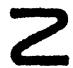
\includegraphics[keepaspectratio]{images/part002_a77d6c20.jpg}}

On the other hand, AB need not be closed when A is closed, even if B is closed too (cf.~§ 4, no. 1, Corollary 1 to Proposition 1).

* For example, in the additive group of the real line \(\mathbf{R}\) , the subgroup \(\mathbf{Z}\) of the rational integers is closed, and so is the subgroup \(\theta\mathbf{Z}\) consisting of all integer multiples \(n\theta\) of an irrational number \(\theta\) ; but the subgroup \(\mathbf{Z} + \theta\mathbf{Z}\) of \(\mathbf{R}\) , which is the set of all real numbers \(m + n\theta\) (where \(m\) and \(n\) take all integer values) is not closed in \(\mathbf{R}\) , as we shall see in Chapter V, § 1.

Again, let A be the subset of the additive group of \(\mathbf{R} \times \mathbf{R}\) which consists of all \((x, y)\) pairs such that \(x \geqslant 0\) and \(0 \leqslant y \leqslant 1 - \frac{1}{x + 1}\) ; and let B be the set of all pairs \((x,0)\) , as x runs through R. A and B are closed, but \(A + B\) is the set of all pairs \((x,y)\) such that \(0 \leqslant y < 1\) , and is not closed in \(R \times R\) .

Let X be a topological space and let f and g be two mappings of X into a topological group G. If f and g are continuous at a point \(x_{0}\) of X, then so are \(\overline{f}^{1}\) and \(fg\) (*), by Theorem 2 of Chapter I, § 2, no. 1. In particular, the continuous mappings of X into G form a subgroup of the group \(\mathbf{G}^{\mathbf{x}}\) of all mappings of X into G.

Again, let \(f\) and \(g\) be two mappings of a set \(\mathbf{X}\) , filtered by a filter \(\mathfrak{F}\) , into a Hausdorff topological group \(\mathbf{G}\) . If \(\lim_{\mathfrak{F}} f\) and \(\lim_{\mathfrak{F}} g\) exist, then so do \(\lim_{\mathfrak{F}} \overline{f}^1\) and \(\lim_{\mathfrak{F}} fg\) , and we have (Chapter I, § 7, no. 4, Proposition 9, Corollary 1)

\[
\lim _ {\mathfrak {F}} \overline {{f}} ^ {- 1} = (\lim _ {\mathfrak {F}} f) ^ {- 1},\tag{1}
\]

\[
\lim _ {\mathfrak {F}} f g = (\lim _ {\mathfrak {F}} f) (\lim _ {\mathfrak {F}} g).\tag{2}
\]

When G is a commutative group, written additively, the axiom (GT') indicates that \((x, y) \to x - y\) is a continuous mapping. If f and g are mappings of a topological space X into G, continuous at a point \(x_{0}\) , then f - g is continuous at this point. The formulas (1) and (2) can be transcribed similarly.
